\chapter{Système de recherche d'information}
\section{Introduction}
Citons d'abord quelques définitions d'un SRI tiré de quelques travaux de recherches, ainsi on va analyser ses composants et puis on va analyser sa performance en utilisant des mesures de performance.

\begin{definition}
    Un système de recherche d'information (SRI) est un système (ensemble des programmes informatiques) qui permet de retrouver les documents pertinents à une requête d'utilisateur en mettant et œuvre des moyens et des techniques, à partir d'une base de documents volumineuse. La requête de l'utilisateur est souvent composé des mots clés \citep{salton1989automatique,approche-semantique}.
\end{definition}

\begin{definition}
	On appelle Système de Recherche d'Information (SRI) un ensemble des programmes, qui sert a interfacer avec l'utilisateur, de prendre les requêtes et de les interpréter afin de faire une recherche dans l'index, appliquer un modèle d’appariement et retourné les documents jugés pertinents a l'utilisateur \citep{amelioration-ri-approche-semantique}.
\end{definition}

\begin{definition}
	Un Système de Recherche d'Information (SRI) permet de récupérer la requête de l'utilisateur, de l'analyser, puis rechercher dans la base documentaire les documents qui correspondent (pertinent) a la requête et de retourner les résultats a l'utilisateur \citep{vsm}.
\end{definition}

\begin{definition}
	Un moteur de recherche est un outil (logiciel) qui permet de collecter des informations, rechercher des informations spécifique sur le Web ou sur un ordinateur personnel, à partir de mots clés et présente les résultats a l'utilisateur \citep{jdn-moteur-de-recherche, mdn-search-engine}.
\end{definition}

\section{Objectif et efficacité}
En général il y a deux catégorie de problème d'un SRI, tel que le problème \emph{centré utilisateur} comme le problème lié a la compréhension et l'analyse de comportement de l'utilisateur; et le problème \emph{centré système} comme le problème lié a la création d'index efficace, traitements des requêtes avec plus de rapidité et efficacité ainsi que le développement d'un algorithme de classement pour améliorer les résultats \citep{modern-ir}.

Mais le problème central d'un SRI est \emph{centré système} qui est de savoir comment satisfaire la besoin d'information de l'utilisateur le plus rapide possible et efficace. C'est un problème plus délicat a résoudre puisqu'il y en a plusieurs facteurs relié a ces performances. De l'autre coté il y a des recherches qui font des analyses de comportement des utilisateurs, ses impactes sur la recherche d’information ainsi que l'utilisation d'un SRI\@. Parmi ces différentes études, il y a celle qui est traité par \citeauthor{ri-sur-le-web} \citep{ri-sur-le-web} dans le cadre des lycéens.

L'objectif d'un SRI est donc de localiser et retourner les documents pertinents par rapport a une requête pour répondre et satisfaire le besoin d'information de l'utilisateur. Le SRI relève donc le défi de rechercher des documents pertinents par rapport au requête de l'utilisateur parmi un très grand volume d'informations \citep{amelioration-ri-approche-semantique}.

L'efficacité d'un SRI est jugé par la capacité de comprendre ce que l'utilisateur veut, ce que l'utilisateur demande a partir de la requête. Ainsi sur sa capacité de fournir les documents pertinents et les classer suivant leurs pertinences par rapport a la requête de l'utilisateur \citep{vsm}. Et aussi la rapidité de récupération des informations et l'accessibilité au niveau de l'interface utilisateur \citep{ir-on-web}.

Dans le cadre de ce devoir, on se focalisera plus sur la performance relié au problème centré système que ceux qui est centré utilisateur.

\section{Élément principaux}
Un Système de Recherche d'Information a deux éléments principaux, tel que la \textit{base de donnée} et l'\textit{algorithme de classement} \citep{approche-semantique}. Ces deux éléments sont indispensables pour un système d'information.

\subsection{Base de données}
\begin{definition}
	Une base de données est une collection organisée d’informations structurées, généralement stockées
	électroniquement dans un système informatique. Généralement contrôlée par un SGBD (Système de Gestion de Base de Données) \citep{oracle-database}.
\end{definition}

\begin{definition}
	Une base de données ou BDD est une collection d’informations organisées afin d’être facilement consultables, gérables et mises à jour. Les bases de données informatiques sont utilisées dans un grand nombre d’entreprises pour stocker, organiser et analyser les données \citep{lebigdata}.
\end{definition}

Pour un SRI, cette base de données est structuré par un expert de base de données (Database Manager). Il est responsable de stockage des documents, des index, ainsi que met en place la relation entre les documents et les index (Fichier inversé). Cette base de données stocke alors l'ensemble de documents utilisé par le système afin de répondre aux besoins de l'utilisateur \citep{vsm-for-arabic-language}.

\subsection{Algorithme de classement}
Un algorithme de classement permet de classer les documents suivant l'ordre de pertinence par rapport a la requête de l'utilisateur. Cette algorithme se charge de calculer la pertinence entre la requête et les documents dans la base de données. L'algorithme de classement souvent utilisé dans le modèle vectoriel est déjà présenté dans la Section~\ref{sec:mesure-similarite}.

\section{Catégorie de recherche}
Tout d'abord, il y a quatre catégories de recherche \citep{ir-on-web} tel que:
\begin{itemize}
	\item \textbf{Recherche simple}: utilise la requête simple
	\item \textbf{Recherche personnalisée}: utilise la requête personnalisée
	\item \textbf{Recherche de dossier}: recherche dans des dossiers
	\item \textbf{Recherche des nouvelles courantes}: utilise la requête des news
	\item \textbf{Contenu web}: suppression des liens mortes
\end{itemize}

\section{Type de moteur de recherche}
Les moteurs de recherche sont catégorisé en deux catégories: moteur de recherche classique qui travaille avec les contenues statique des documents et le moteur de recherche sémantique \citep*{approche-semantique,thesaurus-ir-web}.

Le Tableau~\ref{tab:categorie-sri} illustre les différences entre un moteur de recherche classique et moderne.

\begin{table}[htbp]
	\centering
    \renewcommand{\arraystretch}{1.5} % Specify the line height here
    \begin{tabularx}{\textwidth}{|X|X|}
		\hline
		\textbf{Moteur de recherche classique} & \textbf{Moteur de recherche moderne} \\ 
		\hline
		Nombre de documents inférieur & Nombre de documents supérieur \\
		\hline
		Nombre d'utilisateurs simultanées inférieur & Nombre d'utilisateurs simultanées supérieur \\
		\hline
		Type d’informations simple & Multiple type d'informations \\
		\hline
		Simple, indexation et pondération rapide (Temps, Performance) & Indexation/Clustering/Détermination des pages valués est une challenge \\
		\hline
	\end{tabularx}
	\caption{Catégorie des SRI \citep{ir-on-web}}\label{tab:categorie-sri}
\end{table}

\subsection{Classique ou traditionnel}
Un moteur de recherche classique ou traditionnel traite les documents dont le contenu est statique c'est à dire, le contenu des documents ne change pas au fil du temps. Ce qui implique, que l'étape d'indexation des documents se fait une fois, il n'y a probablement pas de réindexation des documents. Cette approche est souvent utilisé pour la recherche des livres électronique, etc.

\subsection{Sémantique ou moderne}
Ce moteur de recherche provient du traditionnel. Le contenu des documents traités par ce type de SRI sont dynamiques et peuvent varier au fil du temps. Comme par exemple un site WEB qui met a jour fréquemment ses contenus, les suppriment. Dans ce type de moteur de recherche, l'étape d'indexation est de plus en plus complexe, et l'étape de réindexation est nécessaire et souvent periodique pour récupérer les mise a jours des documents. Ce type de moteur de recherche est généralement utilisé pour la recherche sur le WEB\@.

\section{Modèle adopté par un SRI}
Un Système de Recherche d'Information peut adopter un modèle qui se base sur ces trois modèles qui est le modèle \textit{full-text}, le modèle \textit{keyword-based} et le modèle \textit{hypertext} \citep{modern-ir}.
\begin{itemize}
	\item \textbf{Full-text}: ce modèle utilise tous les termes de documents comme un terme d'indexation. C'est à dire pas de discrimination des mots vides. L'indexation et la tache de recherche sont simple, mais peut apporter des bruits.
	\item \textbf{Keyword-based}: ce modèle utilise les mots clés pour représenter les documents, avec la suppression des mots vides. Les termes d'indexation sont donc des mots clés.
	\item \textbf{Hypertext}: ce modèle se base sur des liens, souvent utilisé sur les documents WEB\@.
\end{itemize}

\section{Évaluation d'un SRI}
Il est important d’évaluer un SRI avant d’implémentation pour l'utilisation finale. Cette étape d'évaluation dépend du but finale du SRI\@. En général, il y a trois catégories d'évaluation d'un SRI tel que l'\textit{évaluation fonctionnel} qui fait l'analyse des fonctionnalités du système, l'\textit{évaluation de performance} et l'\textit{évaluation de performance de recherche} \citep{modern-ir}.

Dans l'\emph{évaluation de performance de recherche} troisième catégorie, on utilise des mesures mathématique dont les plus courant sont la \textit{Précision (Precision)} et le \textit{Rappel (Recall)}. C'est souvent dans ce catégorie qui a le plus des difficultés et des défis.

\subsection{Évaluation fonctionnel}
L'évaluation fonctionnel est la première étape d'évaluation d'un SRI\@. Il met en œuvre l'analyse des deux facteurs suivantes:
\begin{itemize}
	\item \textbf{Analyse de fonctionnalités}: analyser tous les fonctionnalités du système une par une pour voir s'il y a bien des failles ou bug. Cette analyse assurera que l'utilisateur finale du système ne tombe pas sur des problèmes de fonctionnalités ou bug (analyse de l'interface graphique si c'est conviviale, l'accessibilité, etc.).
	\item \textbf{Analyse d’erreur}: pour l'analyse d'erreur, on cherche a trouver un moyen pour faire échouer le système, trouver par tous les moyens de faire des traitements pour que le système fait un erreur. Cette analyse permet de voir des erreurs qui ne sont pas identifié avant et de pouvoir les corriger après.
\end{itemize}

\subsection{Évaluation de performance}
L'évaluation de performance permet d'identifier la performance et la robustesse d'un SRI\@. Cette évaluation analyse généralement deux facteurs:
\begin{itemize}
	\item \textbf{Analyse de temps de réponse}: analyser le temps de réponse du système pour répondre a une requête de l'utilisateur. Le but est de minimiser ce temps de réponse pour satisfaire l'utilisateur. Le système doit être rapide en terme de réponse. Avec les machines de plus en plus performants, cet analyse est de moins en moins problématique mais a ne pas ignorer.
	\item \textbf{Analyse de l’espace utilisé}: analyser aussi l'espace disque utiliser par le stockage des index et la collection des documents. Le système doit utiliser le moins d’espace possible, et doit être le plus léger possible.
\end{itemize}

Dans cette évaluation, on analyse aussi la \emph{performance d'indexation} du SRI, l’\emph{interaction avec le Système d'Exploitation}, ainsi que le \emph{délais dans le canaux de communication}.

\subsection{Évaluation de performance de recherche}
L'évaluation de performance de recherche possède un grand défi, est qui est généralement traité par des chercheurs. Le but est de maximiser la précision des résultats de recherche par rapport au requête de l'utilisateur. Pour bien assimiler cette partie, on va illustré la structure de la collection des documents du point de vue du système, qu'on appelle matrice de contingence dans la Figure~\ref{fig:matrice-contingence}.

\begin{figure}[htbp]
	\begin{center}
		\fbox{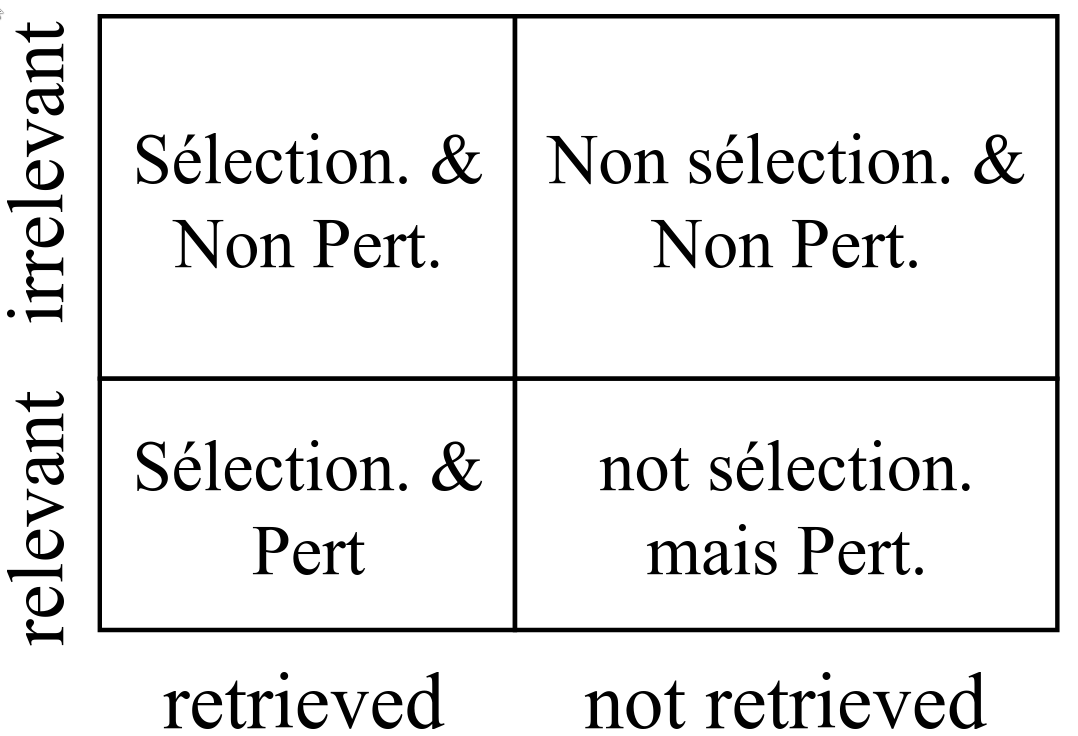
\includegraphics[width=10cm, angle=0]{Figures/SRI/matrice-contingence.png}}
	\end{center}
	\caption{Matrice de contingence \citep{vsm-for-arabic-language}}\label{fig:matrice-contingence}
\end{figure}

Dans ce matrice, il y a quatre catégories tel que:
\begin{itemize}
	\item \textbf{Récupéré et non pertinents}: se sont des documents non pertinents mais jugés pertinent par le système. On cherche a minimiser le nombre des documents dans cette catégorie. On les appelle \emph{faux positif}.
	\item \textbf{Récupéré et pertinents}: se sont des documents pertinents et qui sont sélectionnés par le système. On cherche a maximiser le nombre des documents dans cette catégorie. On l'appelle \emph{vrai positif}.
	\item \textbf{Non récupéré et non pertinents}: se sont des documents non pertinents qui ne sont pas sélectionnés par le système. On cherche aussi a maximiser le nombre des documents dans cette catégorie. On l'appelle \emph{vrai négatif}.
	\item \textbf{Non récupéré et pertinents}: se sont des documents pertinents mais qui ne sont pas récupérer par le système. On cherche a minimiser le nombre des documents dans cette catégorie. On l'appelle \emph{faux négatif}.
\end{itemize}

Dans cette évaluation, on va voir quelques mesures parmi les plus populaires, tel que la \emph{précision}, le \emph{rappel}, et la \emph{F-mesure}. A bien noter que la notion d'ensemble des documents pertinents dans cette évaluation est défini par un expert, qui juge qu'un document est pertinent par rapport a un requête. C'est grâce au connaissance de documents pertinents a l'avance qu'on peut juger le système.

On va illustrer dans la Figure~\ref{fig:precision-recall} la classe des documents pour mieux élaborer la notion de \emph{précision} et \emph{rappel}.
\begin{figure}[htbp]
	\begin{center}
		\fbox{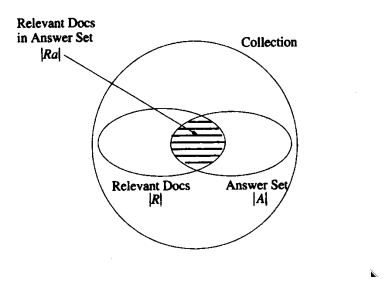
\includegraphics[width=10cm, angle=0]{Figures/SRI/Precision-Recall.png}}
	\end{center}
	\caption{Ensemble des documents \citep{modern-ir}}\label{fig:precision-recall}
\end{figure}

\subsubsection{Précision}
Le précision (precision en anglais) est le rapport du nombre de documents pertinent et le nombre de documents retournés par le système. En d'autre terme, la fraction des documents retournés qui sont pertinents. La précision calcule alors la performance du système a récupérer seulement les documents pertinents \citep*{ir-on-web, evaluation-of-ir-system, vsm-for-arabic-language}. Le but est de maximiser cette valeur.

\[
	Précision = \frac{\textit{Nombre de documents pertinents}}{\textit{Nombre de documents retournés par le système}} = \frac{|Ra|}{|A|}
\]

\subsubsection{Rappel}
Le rappel (recall en anglais) est le rapport entre le nombre de documents pertinents retournés et le nombre total des documents pertinents. En d'autre terme, c'est la fraction des documents pertinents qui sont retournés par le système. Le rappel permet de savoir comment le système a bien récupérer tous les documents pertinents \citep*{ir-on-web, evaluation-of-ir-system, vsm-for-arabic-language}. Le but est de minimiser cette valeur.

\[
	Rappel = \frac{\textit{Nombre de documents pertinents}}{\textit{Nombre de tous les documents pertinents}} = \frac{|Ra|}{|R|}
\]

Il est nécessaire de noter que le rappel n'est efficace dans le cas où la base de données devient large, car le rappel diminue si la base de données augmente. 

\subsection{Exemple de précision et rappel}
Un exemple de calcul de précision et rappel est illustré dans la Figure~\ref{fig:example-prec-rec}.
\begin{figure}[htbp]
	\begin{center}
		\fbox{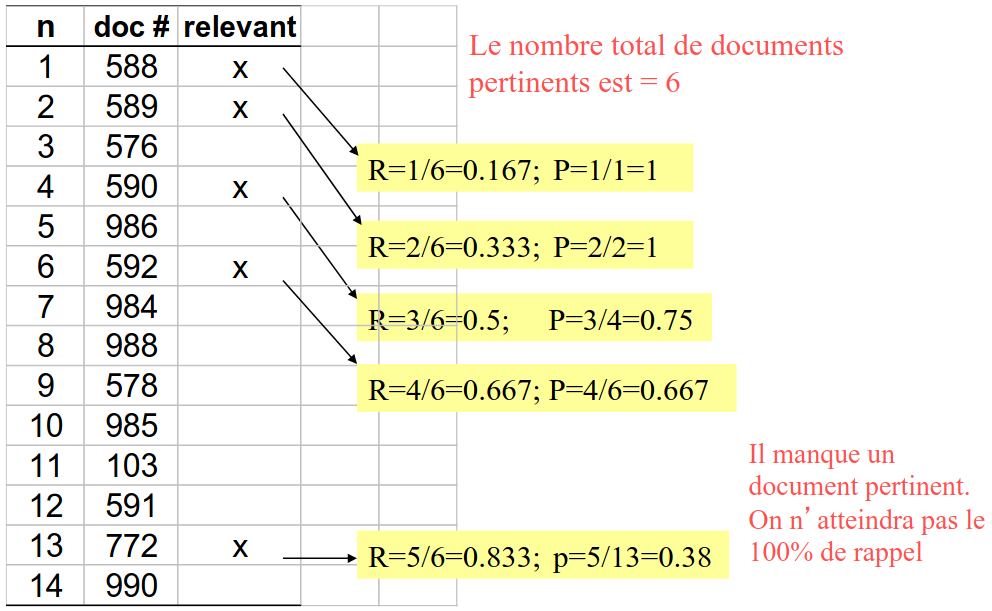
\includegraphics[width=15cm, angle=0]{Figures/SRI/ex-prec-rec.png}}
	\end{center}
	\caption{Exemple de calcule de précision et rappel \citep{evaluation-sri-cours}}\label{fig:example-prec-rec}
\end{figure}

Et la courbe (relation) entre la précision et le rappel est illustré dans la Figure~\ref{fig:example-prec-rec-courbe}
\begin{figure}[htbp]
	\begin{center}
		\fbox{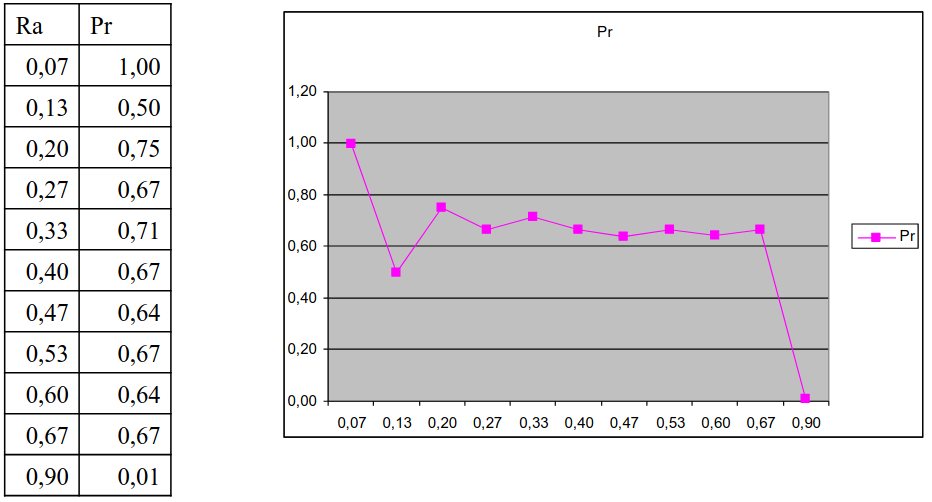
\includegraphics[width=16cm, angle=0]{Figures/SRI/ex-prec-rec-courbe.png}}
	\end{center}
	\caption{Courbe précision-rappel \citep{evaluation-sri-cours}}\label{fig:example-prec-rec-courbe}
\end{figure}

\subsection{Problème de précision et le rappel}
Citons quelques problèmes de la précision et du rappel, comme l'estimation correcte du rappel maximum pour une requête nécessite une connaissance détaillé de tous les documents dans la collection, la précision et le rappel sont deux approche proche qui prend différents aspects de l'ensemble des documents retournés, ainsi ils mesurent l'efficacité a travers une requête traité en groupe ce qui n'est pas adaptable pour un SRI moderne \citep{modern-ir}.

\subsection{Moyenne harmonique}
Cette mesure utilise la précision et le rappel.

\[
	F(j) = \frac{2}{\frac{1}{R(j)} + \frac{1}{P(j)}}
\]
\\Où:\\
\textbf{\textit{R (j)}} est le rappel pour le j-ième document.\\
\textbf{\textit{P (j)}} est la précision pour le j-ième document.\\
\textbf{\textit{F (j)}} est la moyenne harmonique

\subsection{Et d'autres mesures}
D'autres mesure de performance sont utilisés comme \textit{accuracy}, \textit{F-measure}, \textit{E-measure}, \textit{x-precision}, etc. Il y a aussi de notion de silence et bruit \citep*{modern-ir, amelioration-ri-approche-semantique}.

\section{Analyse du moteur de recherche existant}
On peut trouver des thèses malagasy dans différentes moteur de recherche qui existent, mais dans le cadre de ce mémoire, on va analyser quelques uns qui sont populaire (dans le cadre des thèses malagasy) et qui concerne le mieux notre étude.

\subsection{Thèses malgache en ligne}
\emph{Thèse malgache en ligne} \citep{these-malgache-en-ligne} est un SRI orienté WEB spécialisé pour la recherche des thèses soutenues dans les six universités publiques de Madagascar depuis 2006. Actuellement il regroupe actuellement \textbf{31 160} documents, plus précisément des thèses. Ce SRI est hébergé dans le serveur de l'université d'Antananarivo, et est mis en place par les équipes au sein de l'université. Le statistique des documents est dans la Figure~\ref{fig:statistic-tme}, les résultats de recherche ainsi que le système de pagination est illustré dans la Figure~\ref{fig:resultat-tme} et la Figure~\ref{fig:pagination-tme}.

\begin{figure}[htbp]
	\begin{center}
		\fbox{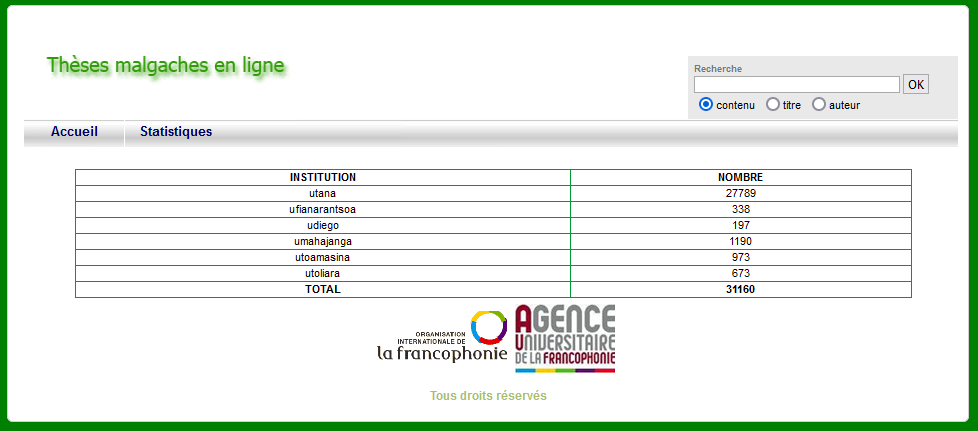
\includegraphics[width=16cm, angle=0]{Figures/SRI/tme-statistics.PNG}}
	\end{center}
	\caption{Statistique des documents \citep{these-malgache-en-ligne}}\label{fig:statistic-tme}
\end{figure}

Ce SRI a pour objectif de faciliter les recherches de thèses, généralement d'auteur malagasy afin d'explorer et de mettre en évidence les fruits de recherche malagasy. Ainsi de faciliter l'accès a ces documents pour les enseignants ainsi que pour les étudiants qui cherche des travaux rattachés a son thème.

L'avantage majeur de ce système est son rapidité en terme de réponse a une requête. Et il est possible de faire une recherche par un titre, auteur et contenu, ainsi que la mise en place de système de pagination pour classer les documents plus pertinents dans la première page, et de naviguer dans les autres pages. Ce SRI classe les résultats suivant l'ordre de pertinence décroissant. L'interface utilisateur est très simple ce qui implique que le chargement de la page est rapide et facile a prendre en main.

Par contre, ce système a quelques lacunes malgré ces avantages. La première problème est l'insuffisance des documents stockés. Vu le nombre d'étudiant ayant soutenu dans les six universités publiques de Madagascar, ce nombre n'est pas suffisant. La deuxième, les documents sont limités pour les établissements publiques, alors qu'il pourra être intéressant d'inclure les documents des établissement privés. La troisième c'est qu'il y a pas de système de catégorisation des documents. Et d'autres problèmes comme le nombre de documents retournés sont nombreux qui implique souvent beaucoup de pagination des résultats (pas de limite de pertinence). Et aussi, il est impossible de voir la résumé d'un document particulier ou afficher une aperçu du document. Et finalement il y a pas de notion de sécurité de document c'est a dire tous les documents sont exposés publiquement en tant qu'utilisateur anonyme.

\begin{figure}[htbp]
	\begin{center}
		\fbox{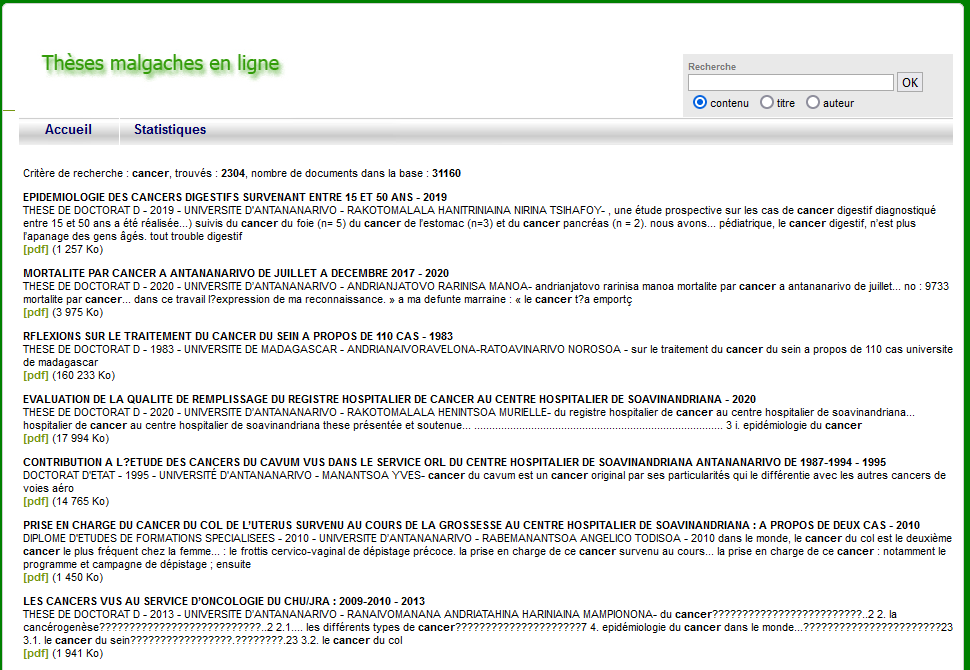
\includegraphics[width=16cm, angle=0]{Figures/SRI/tme-results.PNG}}
	\end{center}
	\caption{Résultat de recherche \citep{these-malgache-en-ligne}}\label{fig:resultat-tme}
\end{figure}

\begin{figure}[htbp]
	\begin{center}
		\fbox{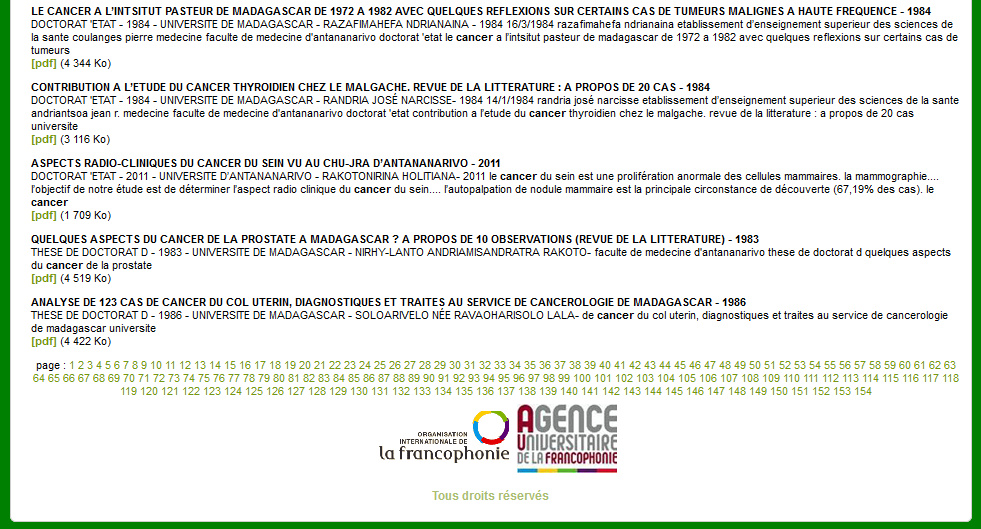
\includegraphics[width=16cm, angle=0]{Figures/SRI/tme-pagination.PNG}}
	\end{center}
	\caption{Système de pagination \citep{these-malgache-en-ligne}}\label{fig:pagination-tme}
\end{figure}

\subsection{Bibliothèques universitaire en ligne}
Les bibliothèques universitaire en ligne n'est plus ni moins qu'une version numérique des bibliothèques. Chaque université publique de Madagascar possède un. En général, c'est pas un SRI complet mais juste une liste des documents disponibles avec un simple recherche généralement sur le titre ou auteur. 

L'objectif est d'exposer des documents pour faciliter l'accès aux étudiants, enseignants ou des personnes voulant accéder a des ressources. Mais en général, ce système fonctionne très bien avec un recherche simple dans le cas des livres par exemple, mas s'avère compliqué pour des recherches avancés. Ainsi les documents sont incomplètes. 

Dans le cadre de recherche des thèses malagasy, ce système est moins efficace que \emph{Thèse malgache en ligne}.

\subsection{Google Scholar, theses.fr et d'autres}
Les géants du moteurs de recherche académique tel que \emph{google scholar}, \emph{Mémoire online}, \emph{HAL}, et d'autres peuvent bien être utilisé pour rechercher des thèses malagasy. Ces systèmes sont performants, puissant en terme d'algorithme utilisés, et stock une grande volume des documents. Certains système propose d’aperçu du document, exportation des bibliographie, liste des articles connexes ainsi qu'un système de sécurité et d'authentification. Il est aussi possible de faire une filtre par année ou par catégorie.

Malgré tous ces atouts, c'est pas suffisant pour les travaux de recherches malagasy. Ces moteurs n'arrivent pas a indexer beaucoup des documents (thèses) malagasy. Par exemple, dans thèses.fr, il y a seulement 41 thèses en cotutelle pour l'université d'Antananarivo \citep{these-fr}. Alors pour rechercher des travaux de recherche malagasy dans ces moteurs est un véritable défi.

\section{Conclusion}
En résumé, un Système de Recherche d'Information ou Moteur de Recherche est un système actuellement indissociable de la vie quotidienne, académique, personnel ou même professionnel. Il a pour but de satisfaire le besoin d'information de l'utilisateur en utilisant des algorithmes et des traitements particulières sur les documents et la requêtes. Un SRI doit passer certains test avant d'être finalement implémenté pour l'utilisation finale. Ces testes sera réalisé pas des experts du domaine, et en utilisant des corpus de test (collection de test) pour pouvoir déterminer la pertinence et la performance du SRI\@. Il y a actuellement beaucoup des moteurs de recherche, certains sont spécialisés dans un domaine spécifique (news, sports, politiques, etc.), mais on a analysé justement quelques un qui est important dans le cadre de ce devoir.
